\section{Conexiones}\label{sec:conexiones}

En esta secci\'on se muestra la interconexi\'on f\'isica entre los
distintos componentes utilizada en el proyecto.

\subsection{Modelo humedad-temperatura}
\begin{center}
\begin{figure}[h]\label{fig:dht22}
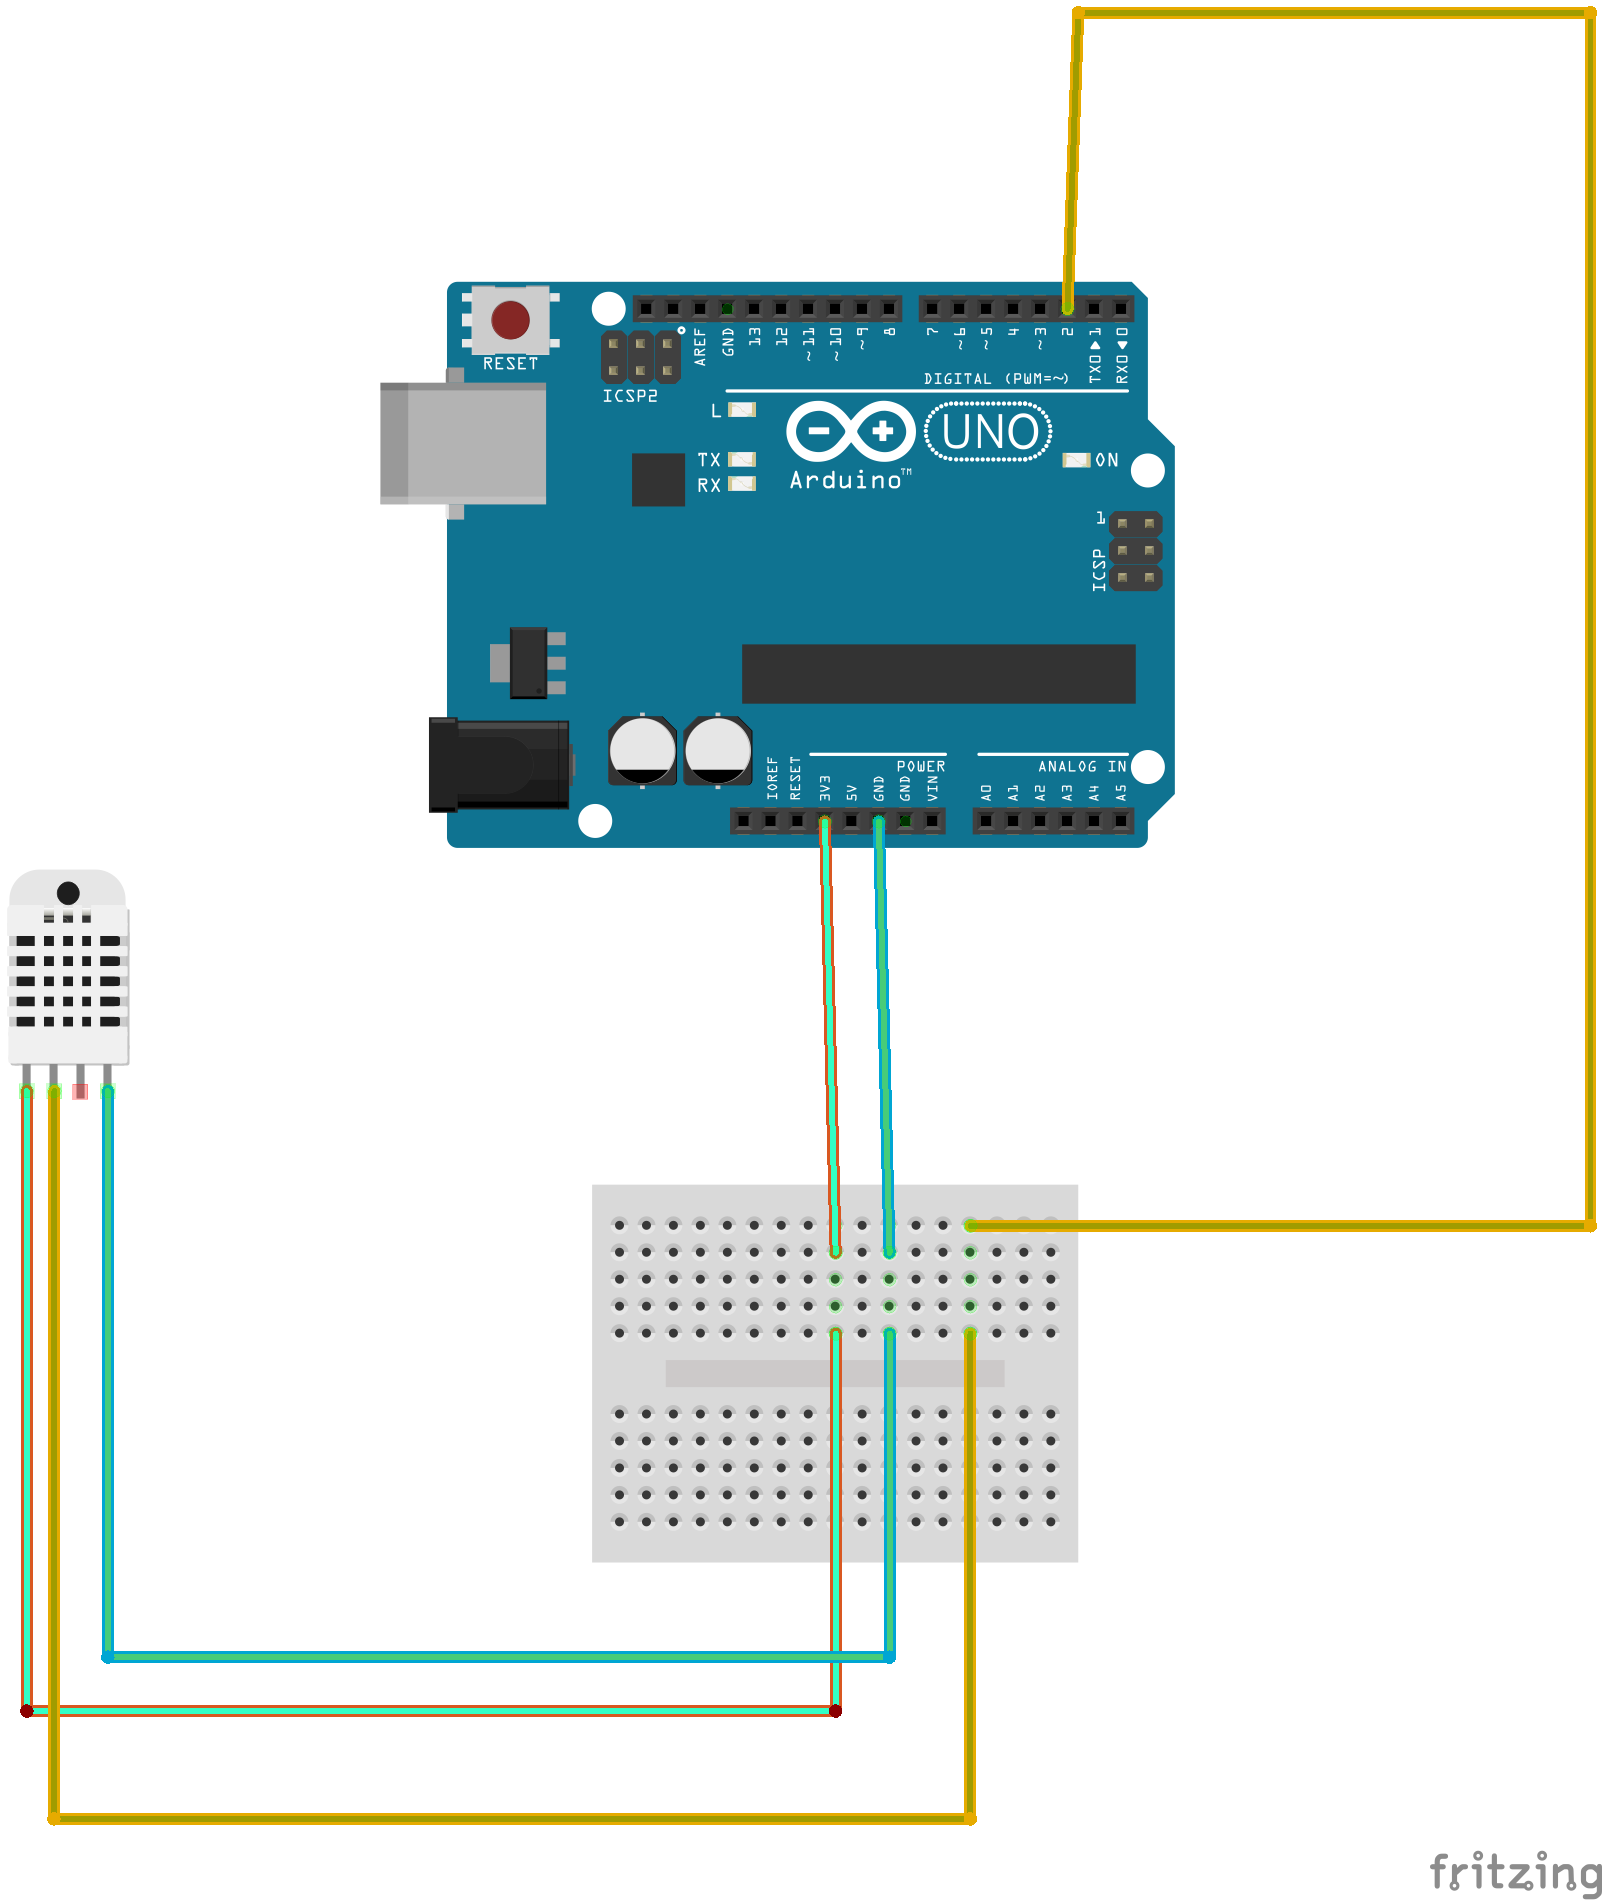
\includegraphics{images/dht22_bb.png}
\caption{Conex\'on entre el sensor DHT22 y ArduinoUNO}
\end{figure}
\end{center}
En la Figura~\ref{fig:dht22} se muestra las conexi\'on f\'isica entre
el ArduinoUno y el sensor de humedad y temperatura DHT22.
Las mediciones llevadas a cabo por el sensor son digitales, raz\'on
por la que se ha utilizado el pin 2 de la placa Arduino, que es
conectado al pin de datos del sensor a trav\'es del cable amarillo.

Los cables azul y verde unen el sensor a tierra y a alimentaci\'on
respectivamente.
El pin 3 del sensor (comenzando por la izquierda) no se utiliza como
se explic\'o en la Secci\'on~\ref{subsec:dht22}.


\subsection{Modelo fotovoltaico}
La conexi\'on f\'isica entre el modelo foltovoltaico y el Arduino Uno
puede ser observado en la figura \ref{fig:bh1750}. Los cables azul y
negro unen el sensor a tierra y a alimentaci\'on, respectivamente.
Al igual que en el modelo anterior, las mediciones de luminosidad son
realizadas de manera digital, por tanto, SDA y SCL est\'an unidos a los puertos A4 y A5, respectivamente.

\begin{center}
\begin{figure}[h]\label{fig:bh1750}
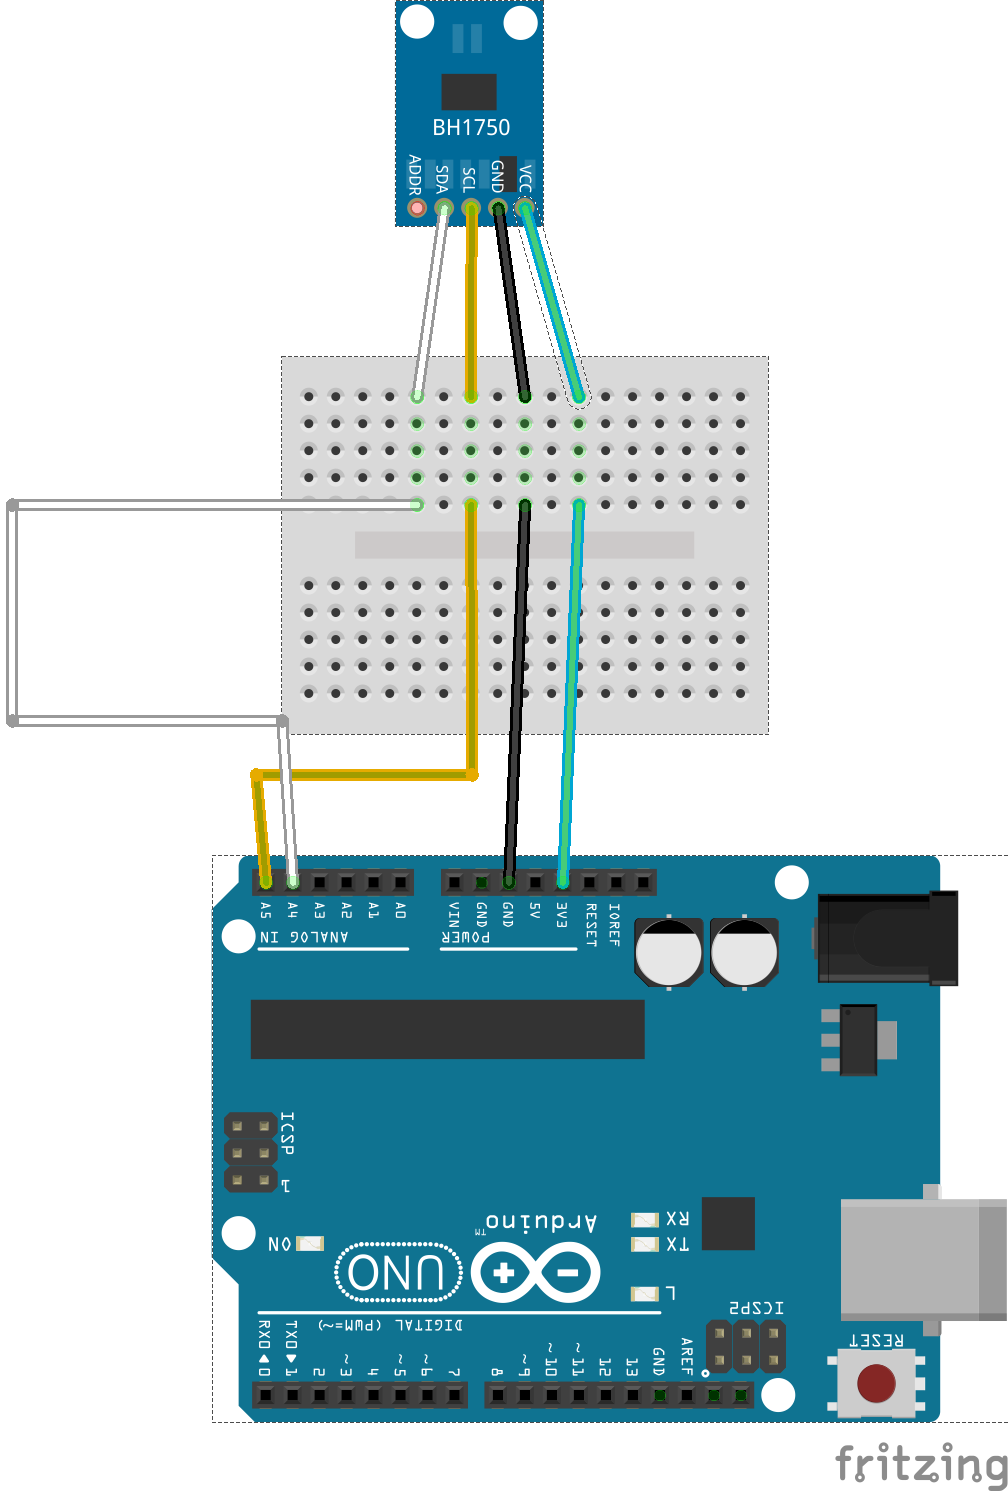
\includegraphics{images/bh1750_bb.png}
\caption{Conex\'on entre el sensor BH1750 y ArduinoUNO}

\end{figure}
\end{center}
\subsection{Modelo Intercomunicaci\'on}\label{sec:mod-intercom}
